 \chapter{Конструкторский раздел}
\label{cha:design}


В данном разделе будут рассмотрены схемы алгоритмов и структура реализации.

\section{Схемы алгоритма Левенштейна}
На рисунке ~\ref{fig:simple} приведена схема стандартного алгоритма умножения матриц.
На рисункt ~\ref{fig:wino} приведеан схема алгоритма Копперсмита--Винограда для умножения матриц.

\begin{figure}
    \centering
    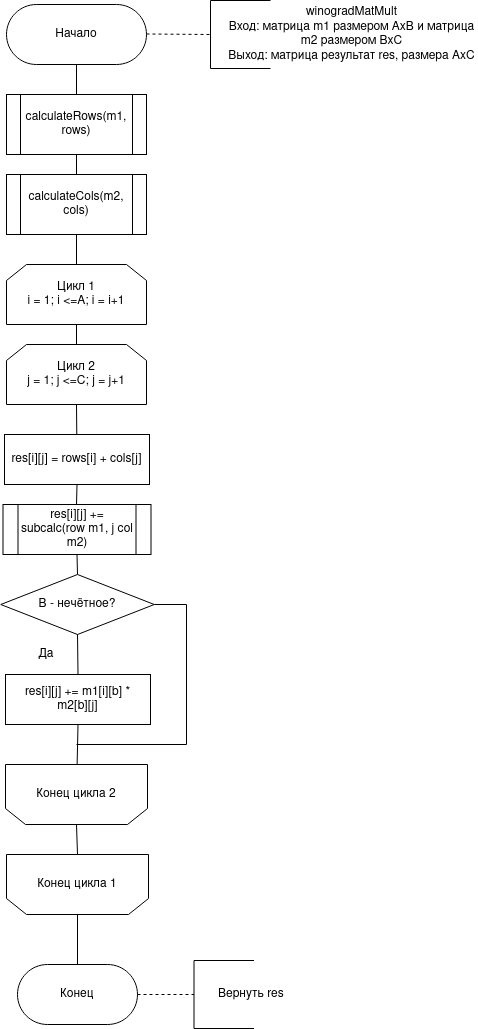
\includegraphics[height=0.65\textheight]{sem-v-aa-master/lab1/tex/inc/schemes/winograd_0.drawio.png}
    \caption{Схема стандратного умножения матриц}
    \label{fig:simple}
\end{figure}

\begin{figure}
    \caption{Схемы алгоритма Копперсмита---Винограда}
    \centering
    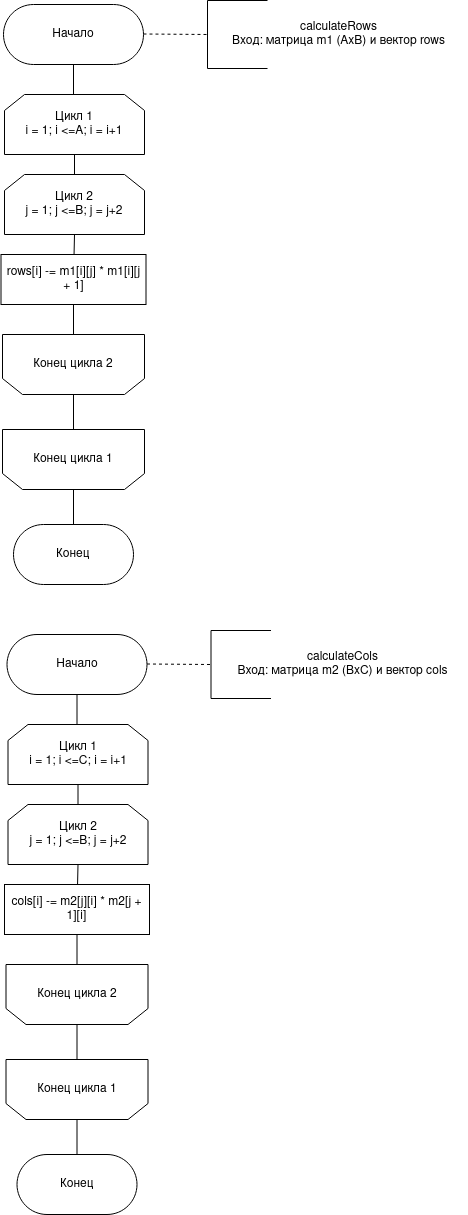
\includegraphics[height=0.8\textheight]{sem-v-aa-master/lab1/tex/inc/schemes/winograd_1.drawio.png}
    \label{fig:wino}
\end{figure}

\section{Модель вычислений}

Для последующего вычисления трудоемкости введем модель вычислений:
\begin{enumerate}[1.]
    \item Операции из списка \ref{eq:operations} имеют трудоемкость $1$. 
    \begin{equation}
        +,-,/,\%,=,\ne,<,>,\leq,\geq,[\;],++,--
        \label{operations}
    \end{equation}
    \item Трудоемкость условного оператора расчитвыается как \ref{eq:conditional}
    \begin{equation}
        f_{if} = f_{условия} + 
        \begin{cases}
            f_{A},& \text{если условие выполняется},\\
            f_{B},& \text{иначе}.
        \end{cases}
        \label{eq:conditional}
    \end{equation}
    \item Трудоемкость цикла рассчитывается как \ref{eq:loop}
    \begin{equation}
        f_{\text{цикл}} = f_{\text{сравнения}} + N \cdot (f_{\text{тела}} + f_{\text{инкремента}} + f_{\text{сравнения}})
        \label{eq:loop}
    \end{equation}
    \item трудоемкость вызова функции равно $0$.
\end{enumerate}

\section{Трудоемкость алгоритмов}
\subsection{Стандартный алгоритм умножения матриц}
Трудоемкость стандартного алгоритма умножения матриц состоит из:
\begin{itemize}
    \item внешнего цикла по $i \in [1..A]$, трудоемкость которого равна \\$f = 2 + A \cdot (2 + f_{\text{body}})$;
    \item Цикла по $j \in [1..C]$, трудоемкость которого равна $f = 2 + C \cdot (2 + f_{\text{body}})$;
    \item Скалярного умножения двух векторов -- цикл по $k \in [1..B]$, трудоемкость которого равна $f = 2 + 10 \cdot B$;
\end{itemize}
Трудоескость стандартного алгоритма равна трудоемкости внешнего цикла, можно вычислить ее, подставив циклы тела \ref{eq:outer_loop}:
\begin{equation}
    f_{\text{base}} = 2 + A \cdot (4 + C \cdot (4 + 10 \cdot B)) = 2 + 4 \cdot A + 4 \cdot A \cdot C + 10 \cdot ABC \approx 10 \cdot ABC
    \label{eq:outer_loop}
\end{equation}

\subsection{Алгоритм Копперсмита--Винограда}
Трудоемкость алгоритма Копперсмита--Винограда состоит из:
\begin{enumerate}[1.]
    \item Создание векторов строк и столбцов \ref{eq:vec}:
    \begin{equation}
        f_{\text{create}} = A + C
        \label{eq:vec}
    \end{equation}
    \item Заполнение вектора строк \ref{eq:rows}:
    \begin{equation}
        f_{\text{rows}} = 3 + \frac{B}{2} \cdot (5 + 12A)
        \label{eq:rows}
    \end{equation}
    \item Заполнение вектора столбцов \ref{eq:cols}:
    \begin{equation}
        f_{\text{cols}} = 3 + \frac{B}{2} \cdot (5 + 12C)
        \label{eq:cols}
    \end{equation}
    \item Цикла заполнения матрицы для четных размеров \ref{eq:loop}:
    \begin{equation}
        f_{\text{loop}} = 2 + A \cdot (4 + C \cdot (11 + \frac{25}{2} \cdot B))
        \label{eq:loop}
    \end{equation}
    \item Цикла, для дополнения умножения суммой последних нечетных строки и столбца, если общий размер нечетный. \ref{eq:last}:
    \begin{equation}
        f_{\text{last}} = \begin{cases}
            2,& \text{четная},\\
            4 + A \cdot (4 + 14C),& \text{нечетная}.
        \end{cases}
        \label{eq:last}
    \end{equation}

\end{enumerate}

Тогда для худшего случая -- то есть нечетного размера матрицы:
\begin{equation}
    f_{\text{worst}} = A + C + 12 + 8A + 5B + 6CB + 25AC + 12,5 \cdot ABC \approx \cdot 12,5ABC.
\end{equation}
Для случая с четным размером получаем \ref{eq:best}:
\begin{equation}
    f_{\text{best}} = A + C + 10 + 4A + 5B + 6CB + 11AC + 12,5ABC \approx 12,5ABC.
    \label{eq:best}
\end{equation}

\subsection{Оптимизированный алгоритм Копперсмита -- Винограда}
Трудоемкость улучшенного алгоритма Копперсмита -- Винограла состоит из: 
\begin{enumerate}[1.]
    \item создание векторов строки и столбцов \ref{eq:op_init}
    \begin{equation}
        f_{\text{init}} = A + C
        \label{eq:op_init}
    \end{equation}
    \item заполнение вектора строки \ref{eq:op_rows_init}
    \begin{equation}
        f_{\text{rows}} = 2 + \frac{B}{2}\cdot(4+8A)
        \label{eq:op_rows_init}
    \end{equation}
    \item заполнение вектора столбцов \ref{eq:op_cols_init}
    \begin{equation}
        f_{\text{cols}} = 2 + \frac{B}{2}\cdot(4+8A)
        \label{eq:op_cols_init}
    \end{equation}
    \item Цикла заполнения матрицы для четных размеров \ref{eq:op_loop_fill}
    \begin{equation}
        f_{\text{loop}} = 2 + \frac{B}{2}\cdot(4+8A)
        \label{eq:op_loop_fill}
    \end{equation}
    \item Цикла для дополнения умножения суммой последней нечетной строки и столбца (в случае нечетной размерности) \ref{eq:con_odd}
    \begin{equation}
        f_last = 3 + \begin{cases}
            0,& \text{четная},\\
            2 + 4 \cdot A + 13 \cdot nm \cdot (4 + 14C),& \text{нечетная}.
        \end{cases}
    \end{equation}
\end{enumerate}

Итого, для худшего случая и лучшего случая: 
\begin{equation}
    f_\text{winograd} = A + C + 10 + 4B + 4BC + 4BA + 8A + 20AC + 9ABC \approx 9ABC.
\end{equation}


\subsection{Структуры данных}
Для матрицы использовалась структура данных с тремя полями: количество строк, столбцов и данные матрицы.

\subsection{Тестирование}
Тестирование будет проведено на двух классах эквивалентности: матриц с четным размером и матриц с нечетным размером. 

\section{Вывод}

Основываясь на теоретическом материале, описанном в аналитическом разделе, были построены схемы обоих алгоритмов умножения матриц. Также были оценены их трудоемкости для лучших и худших случаев.

%%% Local Variables:
%%% mode: latex
%%% TeX-master: "rpz"
%%% End:
